\section{Method}
\label{sec:method}

\subsection{Trashbots as a Probe}
\label{sec:probe}

We used two Trashbot as field probes to study how members of the public read and evaluate a mobile service robot encountered in everyday public space. The Trashbots provided a concrete service that participants could recognize and respond to~\cite{bu2023trash}, while their robotic capabilities invited further interpretation. Their trash-receptacle form suggested a familiar sanitation function, while mobility, onboard camera, and apparently autonomous movement raised questions about what the robot was doing, how it worked, and whether such a system was appropriate or useful in that setting.

This combination made the Trashbots useful for eliciting views about public service robots through actual encounters. Participants could watch a robot move, decide whether to approach or use it, notice its camera and other visible features, and then describe what they understood its actions and presence. The probes therefore grounded participants' accounts in encounter with a functioning service concept.

The two Trashbots followed the same design: a cylindrical trash receptacle mounted on a mobile base, with an onboard camera positioned above the rim (Figure~\ref{fig:Trashbot}). We used a Wizard-of-Oz arrangement throughout the deployments. A researcher controlled each Trashbot from out of view so that people encountered an apparently autonomous mobile service robot. We kept the platform design and operating arrangement consistent across deployment sites.

Using the same probe design across sites allowed us to examine how the setting entered participants' interpretations. The Trashbot's physical form and service concept remained consistent while the surrounding setting changed. We could therefore compare how people read the same service concept in relation to different local conditions.

\begin{figure}[tbp]
    \centering
    \begin{subfigure}[t]{0.54\linewidth}
        \centering
        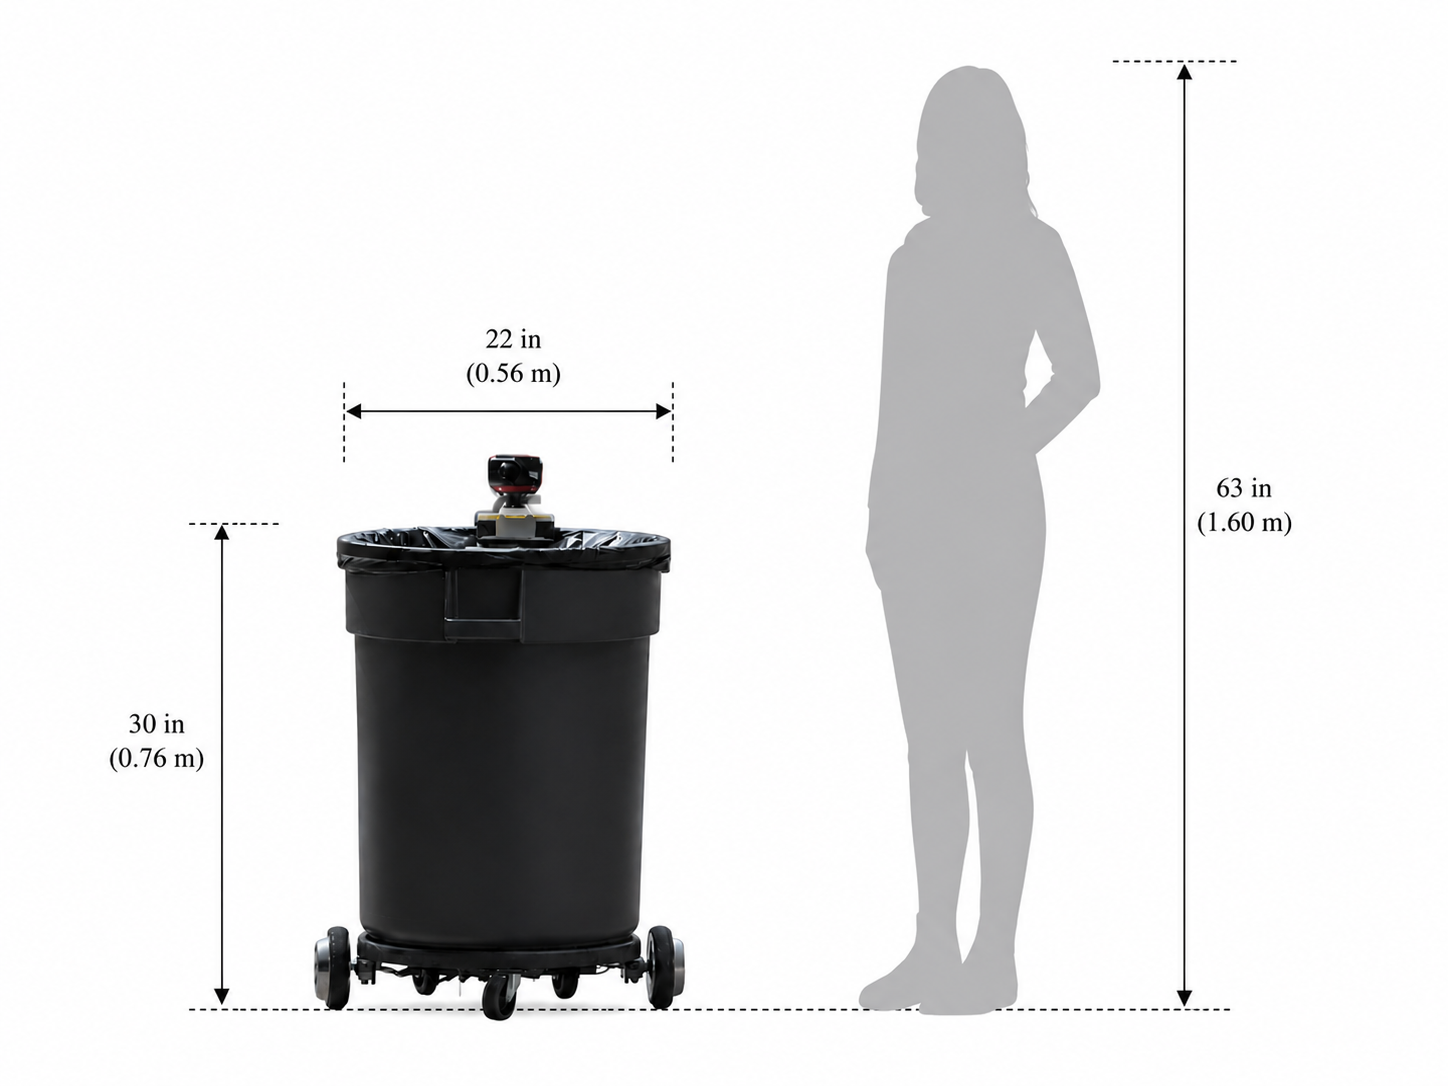
\includegraphics[width=\linewidth, trim=80 35 125 35, clip]{figures/Trashbot_compare.png}
        \caption{Trashbot at scale}
        \label{fig:Trashbot-scale}
    \end{subfigure}\hfill
    \begin{subfigure}[t]{0.43\linewidth}
        \centering
        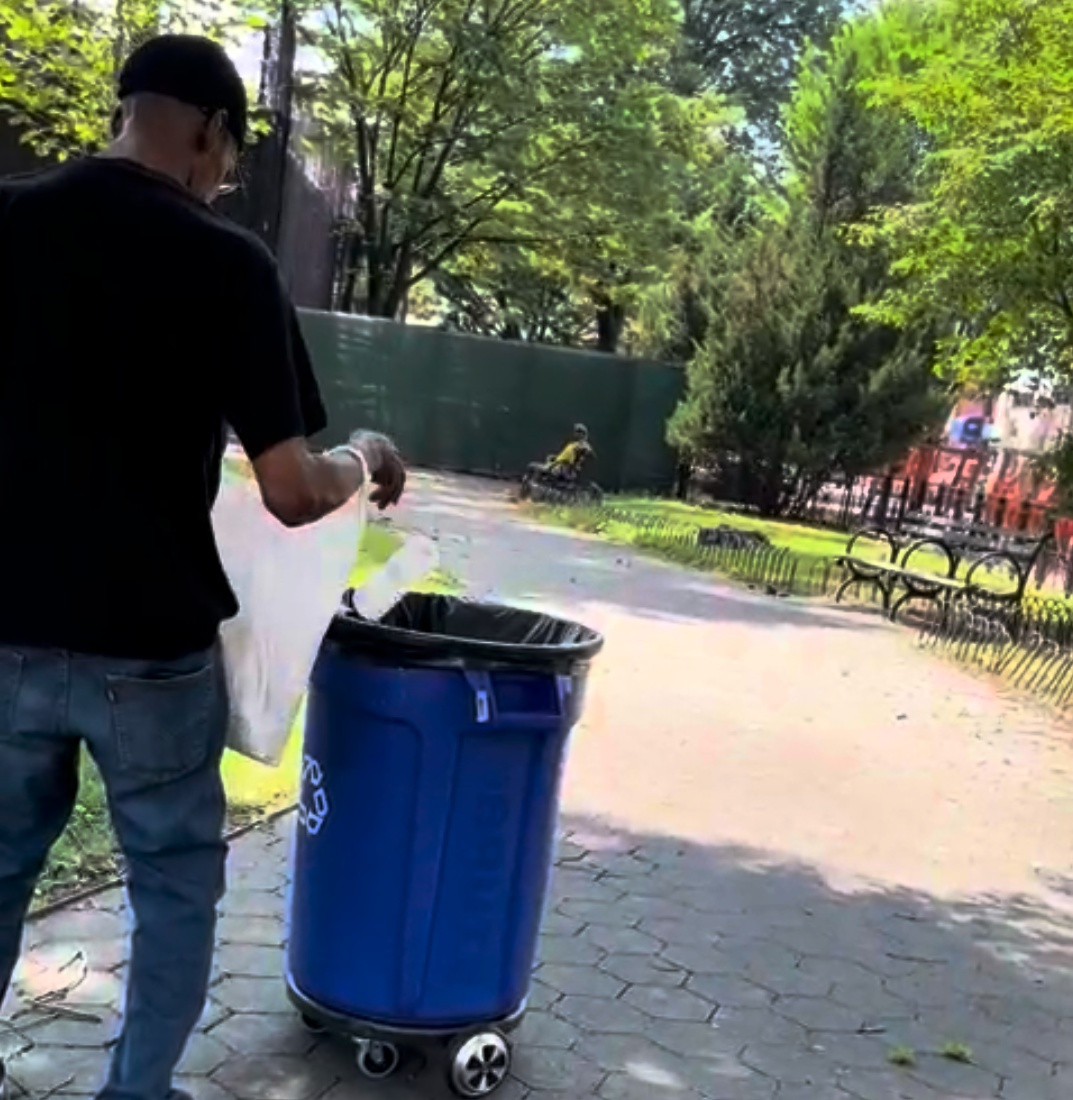
\includegraphics[width=\linewidth]{figures/example_encounter_TP-P03.jpg}
        \caption{Example encounter at Tappen Park}
        \label{fig:Trashbot-encounter}
    \end{subfigure}
    \caption{The Trashbot probe design. (a)~A Trashbot shown at scale next to a person. (b)~A participant at Tappen Park deposits a bag into a Trashbot during an encounter.}
    \Description{Two panels. The left panel shows a Trashbot next to a human silhouette for scale. The Trashbot is a cylindrical trash receptacle on a mobile base with a camera mounted above the rim. The right panel shows a participant at Tappen Park depositing a bag into a Trashbot during a field encounter.}
    \label{fig:Trashbot}
\end{figure}

Prior work has used mobile trash-receptacle robots to study encounters with service robots in public settings~\cite{bu2023trash,brown2024trash,bu2025making}. We use the same approach here to examine how public responses to a service robot vary across deployment sites.
  
\subsection{Deployment and Data Collection}
\label{sec:data-collection}

We deployed Trashbots at five sites across New York City's five boroughs: Tappen Park in Staten Island, Astoria Park in Queens, Little Italy in the Bronx, a cafe at a research institute in Manhattan, and the Brooklyn Navy Yard in Brooklyn. The sites included neighborhood and leisure parks, a commercial corridor, and institutional or commercial campus settings. We selected this set to place the same robot in public settings that differed in spatial organization, patterns of use, and existing service arrangements while remaining within one metropolitan context. Public-park deployments were conducted under a New York City Department of Parks and Recreation research permit. Access to the remaining sites was arranged with the organizations or people responsible for those spaces (see Appendix~\ref{app:sites}). Table~\ref{tab:sites} summarizes the deployment and interview corpus, and Figure~\ref{fig:sites} shows the five deployment locations.

Site selection was purposive rather than experimental. We chose settings that differed in everyday use, sanitation and maintenance arrangements, degree of public access, and institutional context. Feasibility also shaped the final set because each deployment required either a formal research permit or cooperation from the people responsible for the site. 

The sites are not matched conditions. Setting type, local population, degree of public access, sanitation infrastructure, and institutional context vary together across locations, so the study cannot isolate the effect of any one factor. We do not treat site as an independent variable or use these data to estimate neighborhood-level differences in acceptance or behavior. Instead, we use site as context for interpreting what participants believed the Trashbot was, who they thought was responsible for it, what risks they associated with it, and whether they thought it fit the surrounding environment.

The study was approved by our institution's IRB(protocol number omitted for anonymous review). Across the five sites, we conducted 22 field days between April 2025 and August 2026. During each deployment, a Trashbot moved through the accessible public area of the site, approached people, stopped nearby, and continued through the space. People were free to use the receptacle, approach the robot, move away from it, gesture or speak toward it, or ignore it. We did not recruit people before these encounters because doing so could have changed how they interpreted or interacted with the robot.

After an encounter, a researcher approached people and invited them to participate in a short semi-structured interview. Consent was also obtained at that point, after the participant had already encountered the Trashbot. Interviews generally lasted three to five minutes, with longer interviews continuing when participants had more to discuss. The interview guide asked about participants' first impressions, what they thought the Trashbot was doing, how they understood its operation, and their views on having a system like it in the surrounding setting. Follow-up questions asked participants to explain the basis for their judgments when relevant. Interviews were video recorded when consent permitted and otherwise recorded in audio only. We retained and analyzed onboard-camera footage only for participants who permitted recording during consent.

Across the field deployments, the Trashbots encountered approximately 490 people. Several interviews involved pairs or small groups, so interview records and the number of people interviewed are not equivalent. The study involved 115 interview participants in total. The analyzed corpus contained 86 interview records from the five sites. We use the interview record as the unit reported in the quantitative code summaries; one record can therefore contain the views of more than one person.

\begin{table*}[tbp]
\centering
\caption{Trashbot deployment sites and interview corpus.}
\label{tab:sites}
\small
\setlength{\tabcolsep}{3pt}
\renewcommand{\arraystretch}{1.18}
\begin{tabularx}{\linewidth}{@{}
  >{\raggedright\arraybackslash}p{0.11\linewidth}
  >{\raggedright\arraybackslash}p{0.17\linewidth}
  >{\raggedright\arraybackslash}X
  >{\raggedright\arraybackslash}p{0.13\linewidth}
  cc@{}}
  \toprule
  \textbf{Borough} & \textbf{Site} & \textbf{Setting} & \textbf{Dates} &
  \makecell[t]{\textbf{Field}\\\textbf{days}} &
  \makecell[t]{\textbf{Interview}\\\textbf{records}} \\
  \midrule
  Staten Island & Tappen Park & Neighborhood park & Jul 2025 & 4 & 10 \\
  \addlinespace[3pt]
  Queens & Astoria Park & Riverside leisure park & Jul 2025 & 4 & 13 \\
  \addlinespace[3pt]
  Bronx & Little Italy & Commercial corridor & Apr--Oct 2025 & 7 & 32 \\
  \addlinespace[3pt]
  Manhattan & Campus caf\'e & Institutional caf\'e & Jul 2026 & 3 & 16 \\
  \addlinespace[3pt]
  Brooklyn & Brooklyn Navy Yard & Industrial / commercial campus & Jul--Aug 2026 & 4 & 15 \\
  \midrule
  \multicolumn{4}{@{}l}{\textbf{Total}} & \textbf{22} &
  \makecell{\textbf{86}} \\
  \bottomrule
\end{tabularx}

\par\smallskip
\begin{minipage}{\linewidth}
  \footnotesize
  Field days include all deployment days, including days without interview recruitment. Some interview records include pairs or small groups, for 115 people in total. 
\end{minipage}
\end{table*}

Field days and interview recruitment did not always coincide. Some deployments focused on observing encounters or engaging with the surrounding community and produced no interview records. We retain those days in the deployment count because they were part of the field study, while the interview analyses in Sections~\ref{sec:encounters}--\ref{sec:site-sensemaking} use the 86-record analytic corpus.

\begin{figure*}[t]
    \centering
    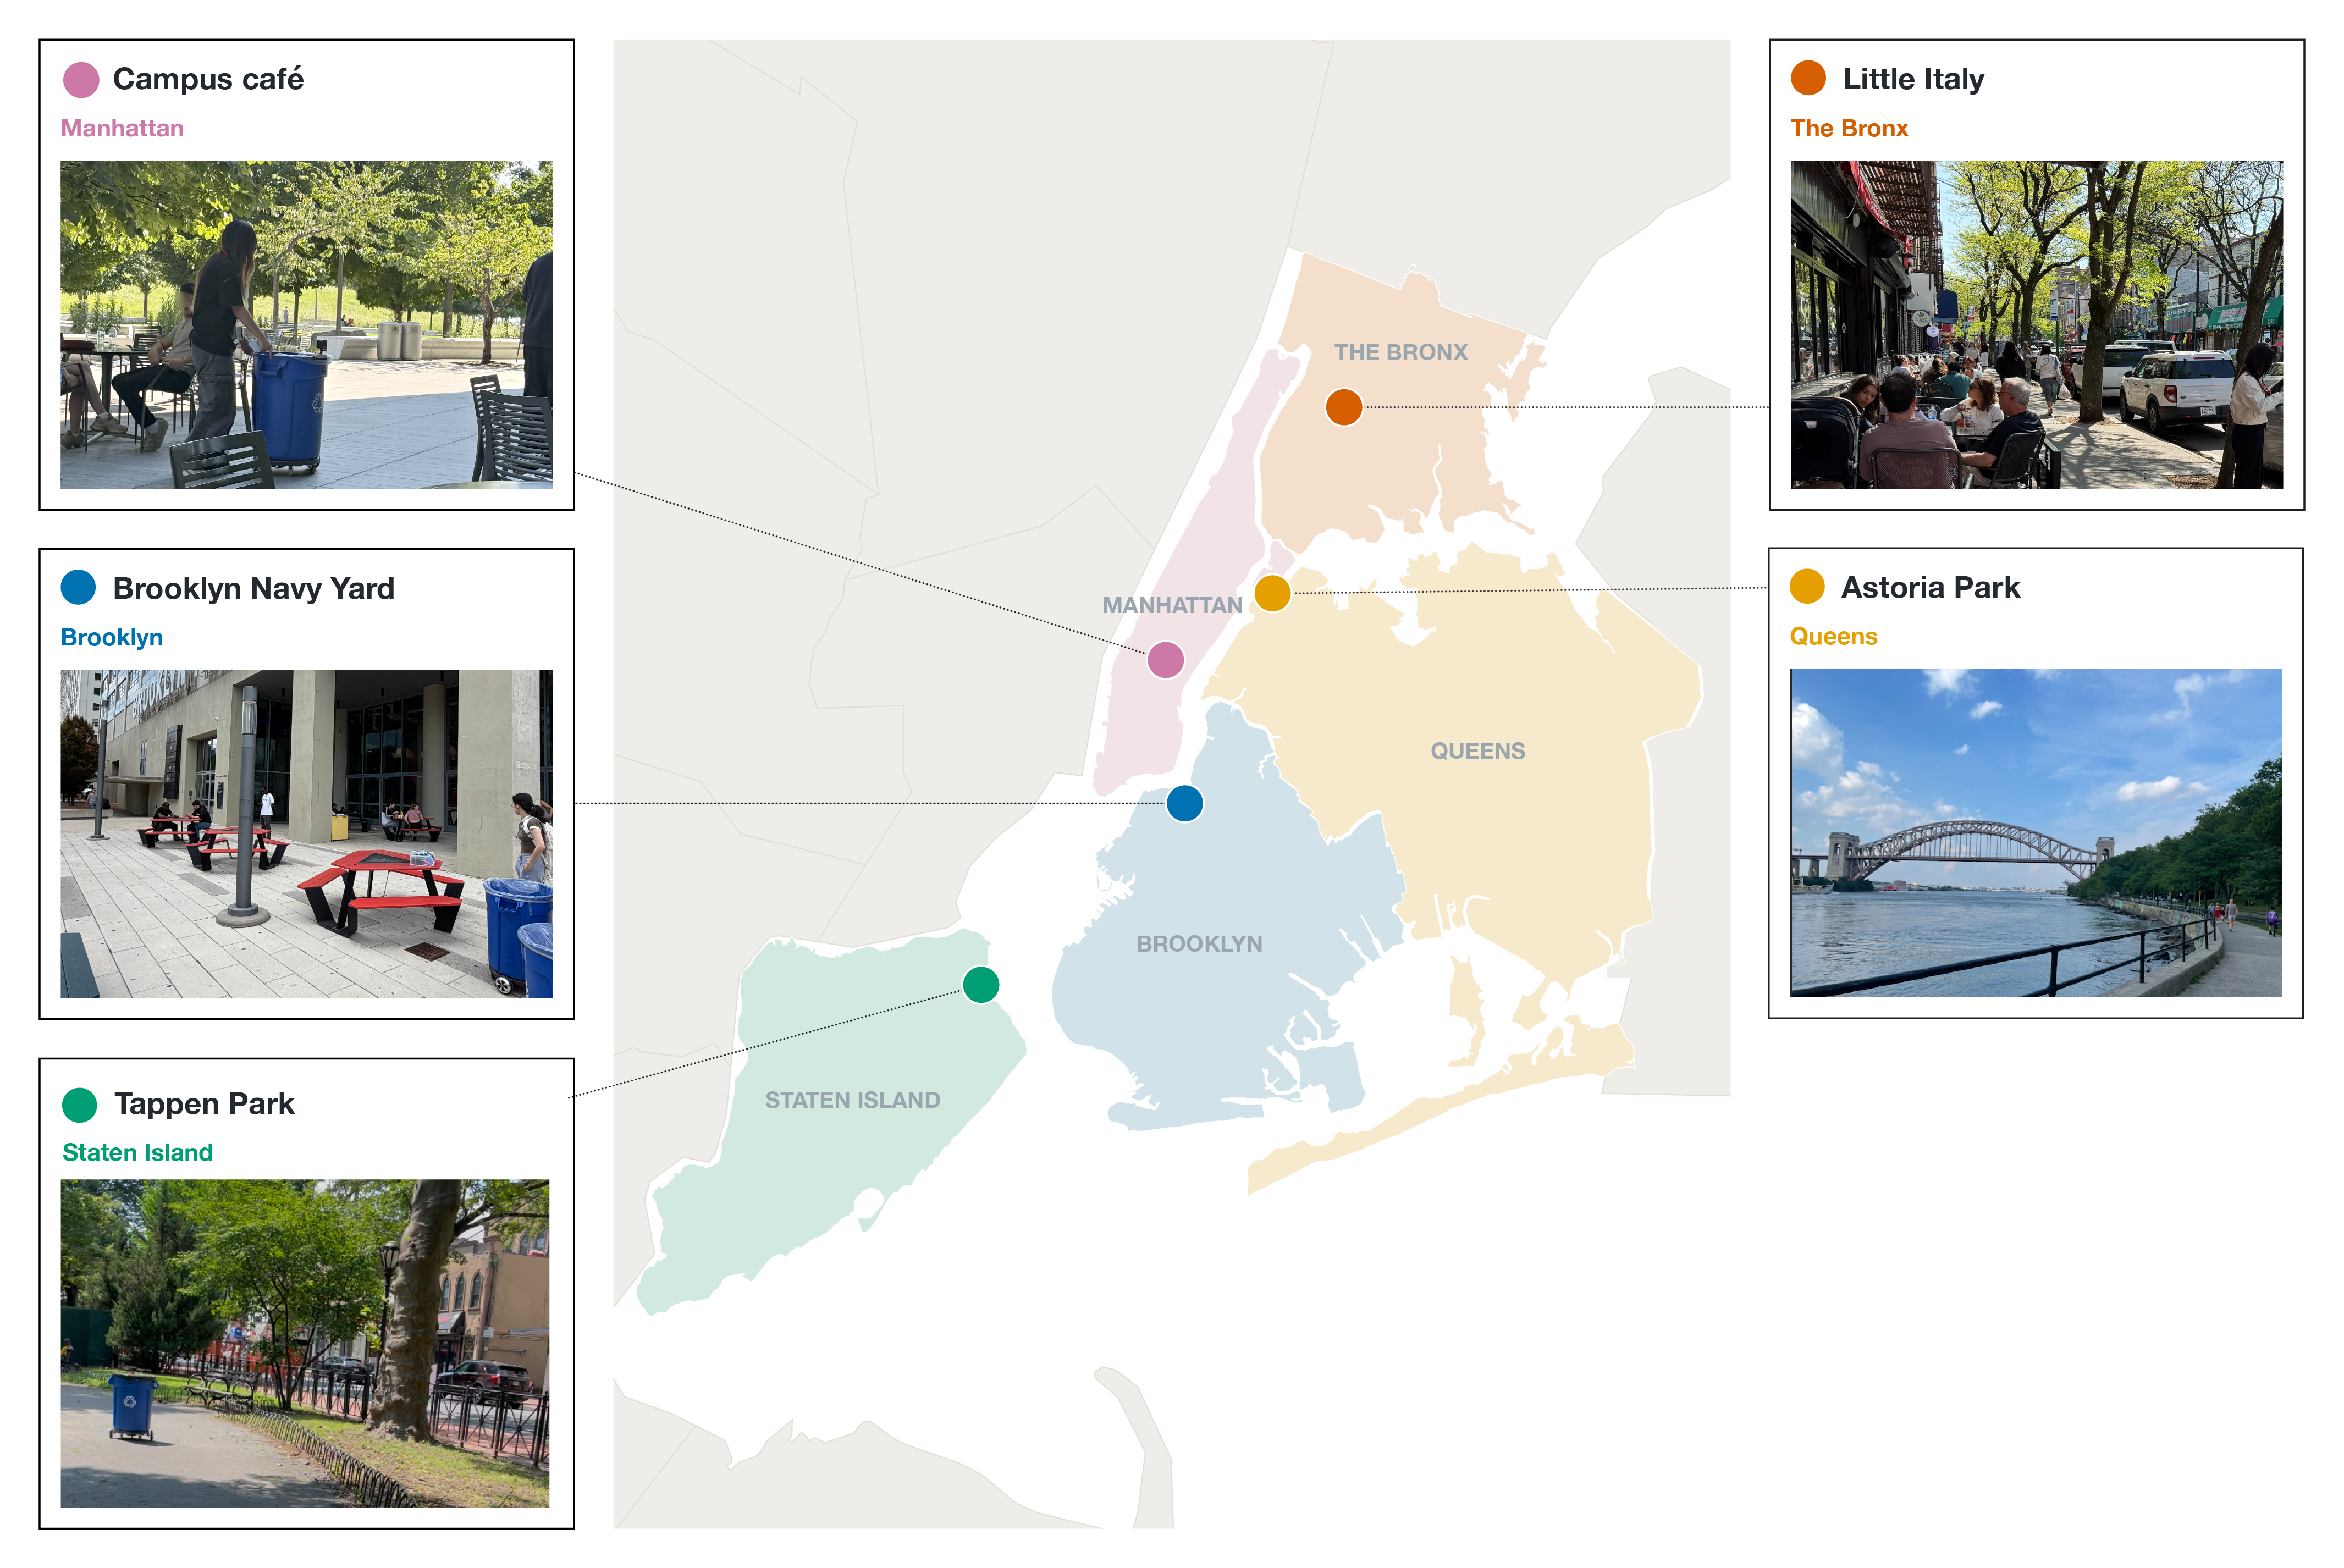
\includegraphics[width=\textwidth]{figures/sites_mapf.png}
    \caption{The five Trashbot deployment sites across New York City's five boroughs. The map shows Tappen Park in Staten Island, Astoria Park in Queens, Little Italy in the Bronx, the Campus caf\'e in Manhattan, and the Brooklyn Navy Yard in Brooklyn.}
    \Description{A map of New York City showing the five Trashbot deployment sites across five boroughs. Tappen Park is in Staten Island, Astoria Park is in Queens, Little Italy is in the Bronx, the campus cafe is in Manhattan, and the Brooklyn Navy Yard is in Brooklyn.}
    \label{fig:sites}
\end{figure*}

\subsection{Data Analysis}
Our analysis draws on records of participants' post-encounter interviews. The interview analysis identified the questions participants sought to resolve and the resources they drew on when interpreting the Trashbot. The interaction analysis characterized how encounters with the robot unfolded in practice. 
\subsubsection{Interview Analysis}
\label{analysis}
Three researchers independently reviewed the interview recordings and working transcripts, each developing a preliminary codebook. They then compared their proposed codes and collaboratively refined them into a shared codebook. The 86 interview records were distributed among the researchers using a round-robin procedure to balance site coverage across coders. Each researcher independently coded their assigned records using the shared codebook.

Following primary coding, we assessed intercoder agreement through independent double-coding of a subset of the interview records \cite{mcdonald2019reliability}. Each researcher coded an additional 15 records originally assigned to another researcher, with these secondary assignments distributed across sites. This procedure yielded 45 double-coded records, representing 52.3\% of the 86 interviews, with overlap covering all three coder pairings. Since the themes are not mutually exclusive, we
compute Cohen’s Kappa coefficient for each theme individually and average the coefficient across
themes. The resulting mean multi-label kappa coefficient is 0.72, which shows substantial agreement~\cite{ComputingInter-RaterReliability}.


\subsubsection{Interaction Analysis}
\label{sec:video-analysis}

Researchers manually reviewed each available onboard-camera recording. We treated the footage as interactional material rather than as a corpus of behavioral variables to be exhaustively coded and counted~\cite{jordan1995interaction}. Reviewers recorded these observations at the level of specific episodes and retained source files and timestamps where available. We used these observations to characterize how encounters unfolded and to identify moments that provided context for participants' later accounts.